\chapter{Lecture 12}

This lecture is about \texttt{Artificial Neural Networks and Self Organizing Maps} where chapter \texttt{ESL Chapter 11.1-11.5
and 14.4} should be looked upon.

\begin{itemize}
  \item Artificial Neural Networks
  \item Autoencoders
  \item Self Organizing Maps
\end{itemize}

\section{Chapter 11.1-11.5}

This chapter is about the Neural Networks, where we get an introduction. How to fit neural networks then talk about issues of the neural networks, for example, the starting values, overfitting, scaling of the inputs, number of hidden units and layers and multiple minima.


\section{Chapter 14.4}

This section is about Self-Organizing Maps

\section{Artificial Neural Networks}

From lecture \cite[p.~6]{lecture12} As a building block in artificial neural networks we introduce the artificial neuron. It takes a weighted sum of the inputs and gives a nonlinear transform as output. This activation function is usually chosen to be a sigmoid function,

\[
    \sigma(v) = \frac{1}{1 + \exp(-v)}
\]

So if we have a network of input layers of $\bm{X} = (x_1, x_2, ... , x_p)$ with hidden layers and output layer(s).

Then the mathematical formulation, for 2 layers, we have

\[
    a_j = \sum_{i = 1}^{P} w_{ji}^{(1)} x_i + w_{j0}^{(1)}
\]

where $j  = 1,...,M$ and the superscript (1) indicates that the corresponding parameters are in the first layer of the network.

Each output is then transformed using a differentiable nonlinear activation function to give

\[
    z_j = h(a_j)
\]

In the context of neural networks, these are called hidden units.

\[
    a_k = \sum_{j = 1}^{M} w_{kj}^{(2)} z_i + w_{k0}^{(2)}
\]

where $k=1,...,K$ and $K$ is total number of outputs. \textbf{For standard regression problems, the activation function is the identity so} $y_k =a_k$, but for binary classification problem, then we use the logistic sigmoid function

\[
    y_k = \sigma (a_k)
\]

So so the mathematical expression is

\[
    f(X) = \sigma\left( \sum_{m=1}^{M}  w_{m}^{(2)} h \left( \sum_{p=1}^{P} w_{mp}^{(1)} x_p + w_{p0}^{(1)}  \right) + w_{0}^{(2)}  \right)
\]

where this can be written to

\[
    f(X) = \sigma\left( \sum_{m=0}^{M}  w_{m}^{(2)} h \left( \sum_{p=0}^{P} w_{mp}^{(1)} x_p   \right)   \right)
\]

This is for one hidden layer feed-forward neural network \cite[p.~7]{lecture12}

For K-class classification ,there are K units at the top, with the k'th unit modelling the probability of class k.

So, we have from \cite[p.~392]{friedman2016elements} that, derived features $Z_m$ are created from linear combinations of the inputs,
and then the target $Y_k$ is modeled as a function of linear combinations of the $Z_m$,

\[
    Z_m = \sigma (\alpha_{0m} + \alpha_m^T X), \quad m=1,...,M
\]

\[
    T_k = \beta_{0k} + \beta_k^T Z, \quad k=1,...,K
\]

\[
    f_k(X) = g_k(T), \quad k=1,...,K
\]

where $Z = (Z_1, Z_2, ... , Z_M)$ and $T = (T_1, T_2, ... , T_K)$

So the softmax function in the output layer is

\[
    g_k (T) = \frac{\exp(T_k)}{\sum_{\ell = 1}^{K} \exp(T_\ell)}
\]

This is the same transform used in K-class logistic regression which produces positive estimates that sum to one.

The unknown parameters are called weights and they should be
fitted to training data by minimizing a loss function $R(W)$.

For the regression we have

\[
    R(W) = \sum_{k=1}^{K} \sum_{i=1}^{N} (y_{ik} - f_k(x_i))^2
\]

and for classification we have

\[
    R(W) = - \sum_{k=1}^{K} \sum_{i=1}^{N} y_{ik} \log f_k (x_i)
\]

The generic approach to minimize $R(W)$ is by gradient descent, called \textit{back-propagation} in this setting. Because of the compositional form of the model, the gradient can be easily derived using the chain rule for differentiation. This can be computed by a forward and backward sweep over the network, keeping track only of quantities local to each unit.

The advantages of back-propagation are its simple, local nature. In the
back propagation algorithm, each hidden unit passes and receives infor-
mation only to and from units that share a connection. Hence it can be
implemented efficiently on a parallel architecture computer. \cite[p.~395]{friedman2016elements}

This is cross-entropy and the output will be a logistic
regression in the hidden layer output.

Computing the derived features $Z_m$, are called hidden units because the values $Z_m$ are not directly observed. In general there can be more than one hidden layer

\begin{figure}[H]
  \centering
  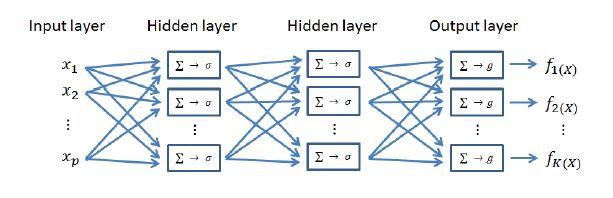
\includegraphics[width=0.9\textwidth]{hiddenlayers}
  \caption{ANN with two hidden layers}\label{fig:hiddenlayers}
\end{figure}

Hidden layers, the number of hidden layers has to be decided. Each
layer extracts features for the next layer allowing for hierarchical
features.

Hidden units, more units mean more flexibility. It is usually better
with too many than too few units. The extra weights can be shrunken
towards zero with regularization

\section{Autoencoders}

Auto encoders are a family of unsupervised neural networks. There are quite a lot of them, e.g. deep auto encoders or those having different regularisation tricks attached--e.g. denoising, contractive, sparse. There even exist probabilistic ones, such as generative stochastic networks or the variational auto encoder. \\

If you want to solve a prediction problem, you will not need auto encoders unless you have only little labeled data and a lot of unlabeled data. Then you will generally be better of to train a deep auto encoder and put a linear SVM on top instead of training a deep neural net.\\

However, they are very powerful models for capturing characteristica of distributions. This is vague, but research turning this into hard statistical facts is currently conducted. Deep latent Gaussian models aka Variational Auto encoders or generative stochastic networks are pretty interesting ways of obtaining auto encoders which provably estimate the underlying data distribution

\section{Some Issues in Training NN}

\subsection{Starting Values}

Note that if the weights are near zero, then the operative part of the sigmoid is roughly linear, and hence the neural network collapses into an approximately linear model.

\subsection{Overfitting}

ANNs are very flexible models with many parameters to tune. Two
techniques are used to avoid overfitting.\\

Cross Validation: Cross validation and evaluation on a separate validation set can be
used to compare different model orders and to tune a regularization
parameter.
Fitting ANNs are time consuming and thus this might take a lot of
time.\\

Early stopping: A simplified approach to regularization often applied to ANN.

During the optimization, of the weights in the model, performance on
a validation set is followed. Instead of having the optimizer finding a
minimum we terminate the iteration when performance on validation
data does not improve anymore. This approach saves a lot of time.

\begin{itemize}
  \item We do not have to repeat the calculations for different CV folds and values on a regularization parameter.
  \item We do not even have to run the optimizer until convergence. We stop when the generalization error starts to increase.
\end{itemize}

The method does not give the best possible model but the technique
is very common when fitting deep networks. \cite[p.~24-25]{lecture10}

\begin{figure}[H]
  \centering
  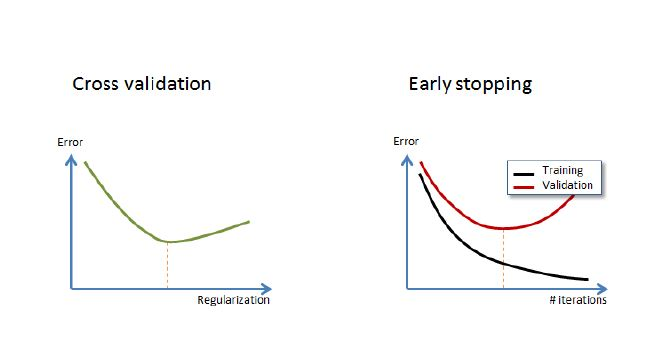
\includegraphics[width=0.9\textwidth]{ANNoverfitting}
  \caption{Cross-validation vs early stopping}\label{fig:ANNoverfitting}
\end{figure}


\section{Self Organizing Maps}

\begin{itemize}
  \item Unsupervised clustering
  \item Projection of data to a low dimensional space
  \item Observations are grouped into clusters much like K-means clustering
  \item The clusters have neighbors in a one or two dimensional grid.
  \item Neighbor clusters are enforced to lay close to each other also in feature space
  \item This creates a mapping of data down to one or two dimensions.
  \item Great for visualization
  \begin{itemize}
    \item Exploratory data analysis
    \item Overview of large amounts of text documents
  \end{itemize}
\end{itemize}

The observation $x_i$ are processed one at a time. We find the closest prototype $m_j$ to $x_i$ in Euclidean distance in $\mathbb{R}^p$.

The neighbors are defined to be all, such that the distance is small.


More about this on \cite[p.~528]{friedman2016elements}
